\section{Preventivo}\label{sdl}
In questa sezione vengono presentate, per ciascuna fase, le ore di impiego dei ruoli preventivate, la ripartizione di tali ore tra i componenti del gruppo e i costi che derivano da tale suddivisione. \\
Si ricorda che i costi delle fasi di \fA e di \fAD sono a carico del \gloxy{fornitore} e di conseguenza non saranno considerate nel preventivo finale.
\subsection{Dettaglio fasi rendicontate}
%----------------------------------------------------------------------------------------------
%----------------------------------------------------------------------------------------------
\subsubsection{Fase di \fPAt}\label{prfPAt}
\subsubsubsection{Suddivisione del lavoro}
Nella fase di \fPA, ciascun componente dovrà rivestire i seguenti ruoli:
%tabella suddivisione
\begin{table}[h]
\begin{center}
\begin{tabular}{|c|c|c|c|c|c|c|c|}
\hline Nome & Re & Am & An & Pt & Pr & Ve & Ore totali\\
\hline
\gma & - & - & - & 25 & - & 1 & 26 \\
\ao & - & - & - & 25 & - & 1 & 26 \\
\mb & - & - & - & 25 & - & - & 25 \\
\dm & - & - & - & 25 & - & 1 & 26 \\
\gmi & - & - & - & 10 & - & 17 & 27 \\
\sm & 3 & 4 & - & 15 & - & 4 & 26 \\
\fv & - & - & 8 & - & - & 21 & 29 \\
\hline Totale ruoli & 3 & 4 & 8 & 125 & - & 45 & 185 \\
\hline
\end{tabular}
\caption{Ore per ruolo - Fase di \fPAt}
\end{center}
\end{table}
\FloatBarrier
I valori vengono riassunti nel seguente grafico:
\begin{figure}[htbp]
\centering
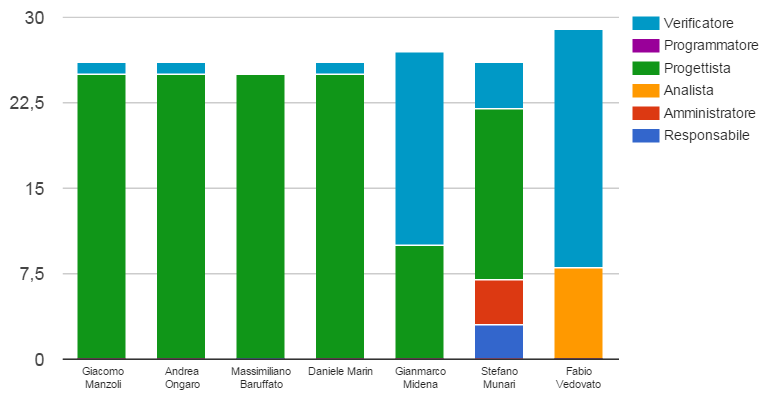
\includegraphics[width=\textwidth]{../immagini/nuoviGrafici/componenti/oreCompFaseProgArc.png}
\caption{Ore per componente - Fase di \fPAt}
\end{figure}
\FloatBarrier
\subsubsubsection{Prospetto economico} \label{prospettofPAt}
Il totale delle ore di lavoro di ogni ruolo e il relativo costo vengono riportati nella seguente tabella:
\begin{table}[h]
\begin{center}
\begin{tabular}{|m{3cm}|m{1.5cm}|m{1.5cm}|}
\hline Ruolo & Ore & Costo (\euro) \\
\hline
\rRPt & 3 & 90 \\
\rAPt & 4 & 80 \\
\rAt & 8 & 200 \\
\rPt & 125 & 2750 \\
\rpt & 0 & 0 \\
\rVt & 45 & 675 \\
\hline
Totale & 185 & 3795 \\
\hline
\end{tabular}
\caption{Prospetto economico - Fase di \fPAt}
\end{center}
\end{table}
\FloatBarrier
I seguenti grafici illustrano rispettivamente come ciascun ruolo abbia influito sul totale delle ore e dei costi della fase di \fPAt.
%grafico a torta dei costi e delle ore
\begin{figure}[h]
\centering
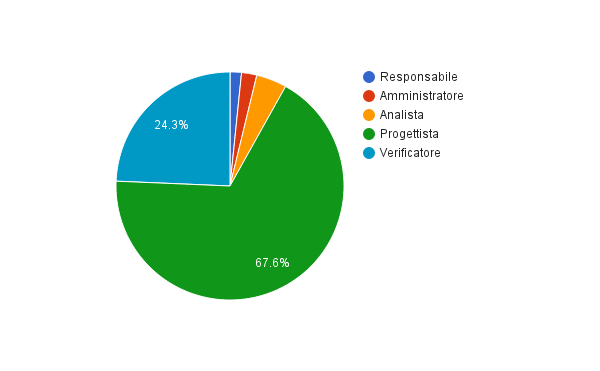
\includegraphics[width=0.9\textwidth]{../immagini/nuoviGrafici/oreFaseProgArc.png}
\caption{Ore per ruoli - Fase di \fPAt}
\end{figure}
\begin{figure}[h]
\centering
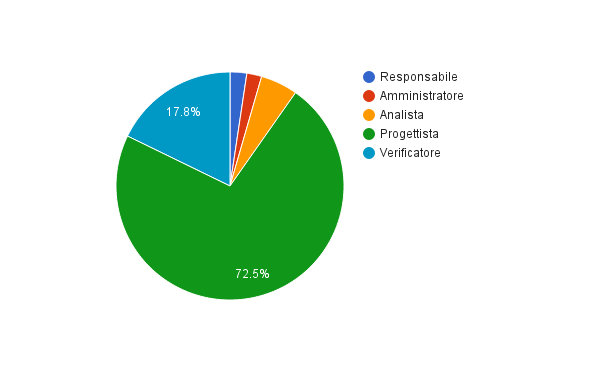
\includegraphics[width=0.9\textwidth]{../immagini/nuoviGrafici/costoFaseProgArc.png}
\caption{Costi per ruoli - Fase di \fPAt}
\end{figure}
\FloatBarrier
%----------------------------------------------------------------------------------------------
\subsubsection{Fase di \fPDt}
\subsubsubsection{Suddivisione del lavoro}
Nella fase di \fPD, ciascun componente dovrà rivestire i seguenti ruoli:
%tabella suddivisione
\begin{table}[h]
\begin{center}
\begin{tabular}{|c|c|c|c|c|c|c|c|}
\hline Nome & Re & Am & An & Pt & Pr & Ve & Ore totali\\
\hline
\gma & - & 4 & 2 & - & - & 20 & 26 \\
\ao & - & - & - & 24 & - & 1 & 25 \\
\mb & 3 & - & - & 8 & - & 16 & 22 \\
\dm & - & - & - & 24 & - & 2 & 26 \\
\gmi & - & - & - & 24 & - & - & 24 \\
\sm & - & - & - & 24 & - & 2 & 26 \\
\fv & - & - & - & 24 & - & - & 24 \\
\hline Totale ruoli & 3 & 4 & 2 & 128 & - & 41 & 178 \\
\hline
\end{tabular}
\caption{Ore per ruolo - Fase di \fPDt}
\end{center}
\end{table}
\FloatBarrier
I valori vengono riassunti nel seguente grafico:
\begin{figure}[htbp]
\centering
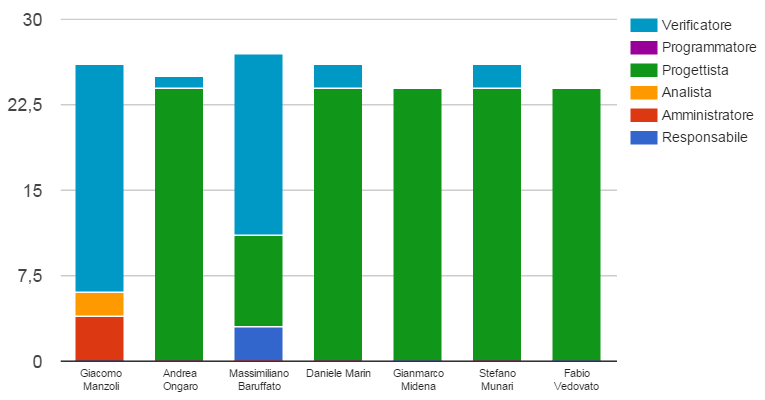
\includegraphics[width=\textwidth]{../immagini/nuoviGrafici/componenti/oreCompFaseProgDet.png}
\caption{Ore per componente - Fase di \fPDt}
\end{figure}
\FloatBarrier
\subsubsubsection{Prospetto economico}\label{prospettofPDt}
Il totale delle ore di lavoro di ogni ruolo e il relativo costo vengono riportati nella seguente tabella:
\begin{table}[h]
\begin{center}
\begin{tabular}{|m{3cm}|m{1.5cm}|m{1.5cm}|}
\hline Ruolo & Ore & Costo (\euro) \\
\hline
\rRPt & 3 & 90 \\
\rAPt & 4 & 80 \\
\rAt & 2 & 50 \\
\rPt & 128 & 2816 \\
\rpt & 0 & 0 \\
\rVt & 41 & 615 \\
\hline
Totale & 178 & 3651 \\
\hline
\end{tabular}
\caption{Prospetto economico - Fase di \fPDt}
\end{center}
\end{table}
\FloatBarrier
I seguenti grafici illustrano rispettivamente come ciascun ruolo abbia influito sul totale delle ore e dei costi della fase di \fPD.
%grafico a torta dei costi e delle ore
\begin{figure}[h]
\centering
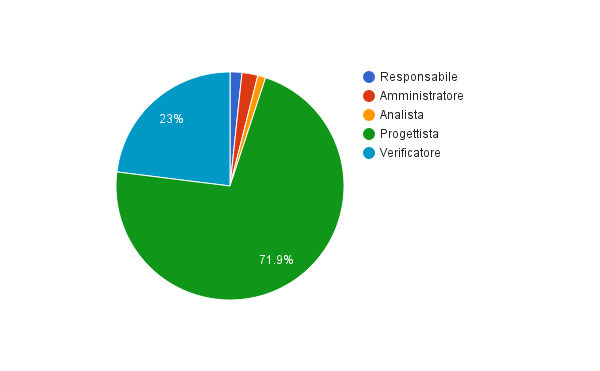
\includegraphics[width=0.9\textwidth]{../immagini/nuoviGrafici/oreFaseProgDet.png}
\caption{Ore per ruoli - Fase di \fPDt}
\end{figure}
\begin{figure}[h]
\centering
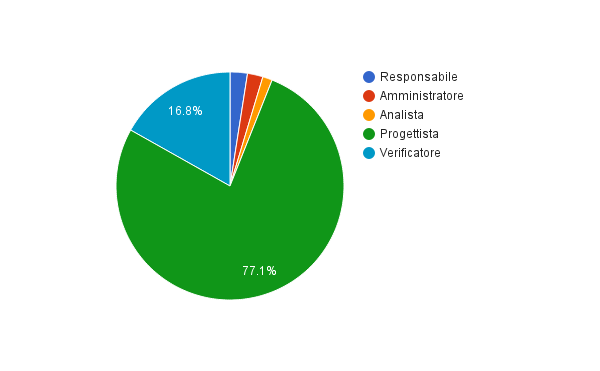
\includegraphics[width=0.9\textwidth]{../immagini/nuoviGrafici/costoFaseProgDet.png}
\caption{Costi per ruoli - Fase di \fPDt}
\end{figure}
\FloatBarrier
%----------------------------------------------------------------------------------------------
\subsubsection{Fase di \fCt} \label{prospettoCod}
\subsubsubsection{Suddivisione del lavoro}
Nella fase di \fC, ciascun componente dovrà rivestire i seguenti ruoli:
%tabella suddivisione
\begin{table}[h]
\begin{center}
\begin{tabular}{|c|c|c|c|c|c|c|c|}
\hline Nome & Re & Am & An & Pt & Pr & Ve & Ore totali\\
\hline
\gma & - & - & - & 10 & 23 & 5 & 38 \\
\ao & - & - & - & - & 35 & 4 & 39 \\
\mb & - & - & 3 & 10 & 26 & - & 39 \\
\dm & - & - & - & - & 22 & 16 & 38 \\
\gmi & 6 & - & 3 & - & - & 29 & 38 \\
\sm & - & - & - & 10 & 10 & 18 & 38 \\
\fv & - & 2 & - & 10 & - & 25 & 37 \\
\hline Totale ruoli & 6 & 2 & 6 & 40 & 116 & 97 & 267 \\
\hline
\end{tabular}
\caption{Ore per ruolo - Fase di \fCt}
\end{center}
\end{table}
\FloatBarrier
I valori vengono riassunti nel seguente grafico:
\begin{figure}[htbp]
\centering
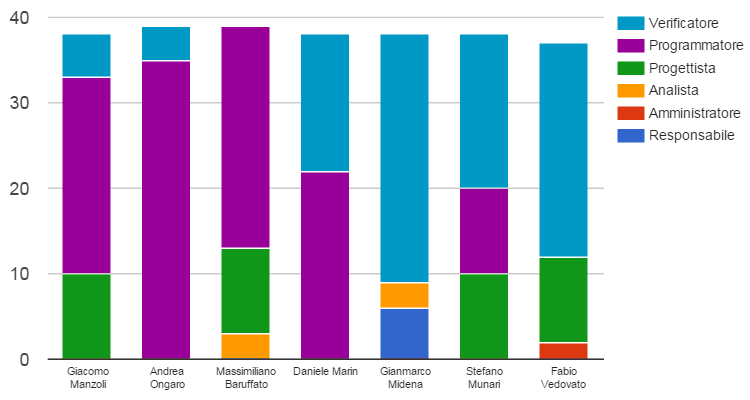
\includegraphics[width=\textwidth]{../immagini/nuoviGrafici/componenti/oreCompFaseCodifica.png}
\caption{Ore per componente - Fase di \fCt}
\end{figure}
\FloatBarrier
\subsubsubsection{Prospetto economico}
Il totale delle ore di lavoro di ogni ruolo e il relativo costo vengono riportati nella seguente tabella:
\begin{table}[h]
\begin{center}
\begin{tabular}{|m{3cm}|m{1.5cm}|m{1.5cm}|}
\hline Ruolo & Ore & Costo (\euro) \\
\hline
\rRPt & 6 & 180 \\
\rAPt & 2 & 40 \\
\rAt & 6 & 150 \\
\rPt & 40 & 880 \\
\rpt & 116 & 1740 \\
\rVt & 97 & 1455 \\
\hline
Totale & 267 & 4445 \\
\hline
\end{tabular}
\caption{Prospetto economico - Fase di \fCt}
\end{center}
\end{table}
\FloatBarrier
I seguenti grafici illustrano rispettivamente come ciascun ruolo abbia influito sul totale delle ore e dei costi della fase di \fC.
%grafico a torta dei costi e delle ore
\begin{figure}[h]
\centering
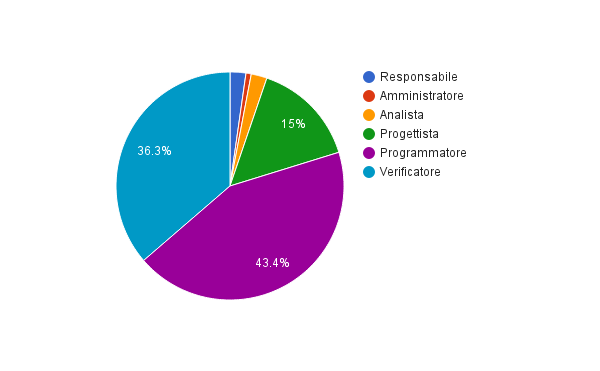
\includegraphics[width=0.9\textwidth]{../immagini/nuoviGrafici/oreFaseCodifica.png}
\caption{Ore per ruoli - Fase di \fCt}
\end{figure}
\begin{figure}[h]
\centering
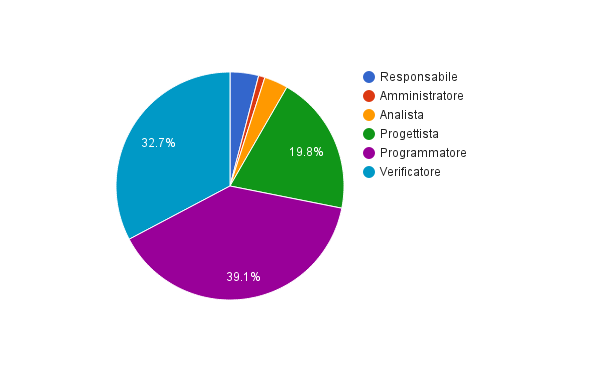
\includegraphics[width=0.9\textwidth]{../immagini/nuoviGrafici/costoFaseCodifica.png}
\caption{Costi per ruoli - Fase di \fCt}
\end{figure}
\FloatBarrier
%----------------------------------------------------------------------------------------------
\subsubsection{Fase di \fVVt} \label{prospettoVer}
\subsubsubsection{Suddivisione del lavoro}
Nella fase di \fVV, ciascun componente dovrà rivestire i seguenti ruoli:
%tabella suddivisione
\begin{table}[h]
\begin{center}
\begin{tabular}{|c|c|c|c|c|c|c|c|}
\hline Nome & Re & Am & An & Pt & Pr & Ve & Ore totali\\
\hline
\gma & - & - & - & 6 & - & 5 & 11 \\
\ao & - & - & 2 & - & - & 9 & 11 \\
\mb & - & - & - & 4 & - & 6 & 10 \\
\dm & 3 & - & - & - & - & 7 & 10 \\
\gmi & - & - & - & - & 3 & 8 & 11 \\
\sm & - & 2 & - & - & - & 9 & 11 \\
\fv & - & - & - & - & 9 & 2 & 11 \\
\hline Totale ruoli & 3 & 2 & 2 & 10 & 12 & 46 & 75 \\
\hline
\end{tabular}
\caption{Ore per ruolo - Fase di \fVVt}
\end{center}
\end{table}
\FloatBarrier
I valori vengono riassunti nel seguente grafico:
\begin{figure}[htbp]
\centering
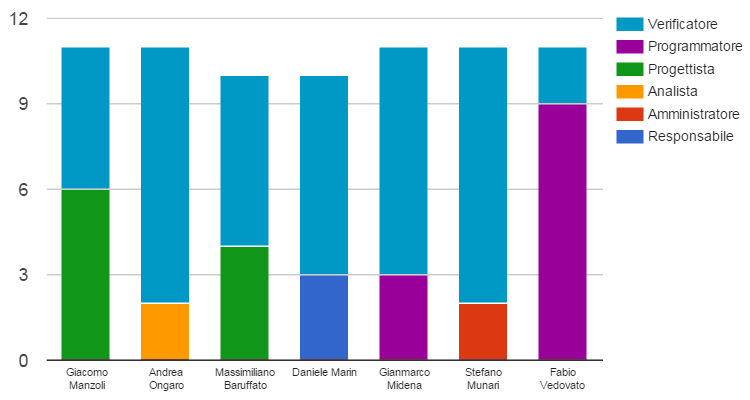
\includegraphics[width=\textwidth]{../immagini/nuoviGrafici/componenti/oreCompFaseVerifica.png}
\caption{Ore per componente - Fase di \fVVt}
\end{figure}
\FloatBarrier
\subsubsubsection{Prospetto economico}
Il totale delle ore di lavoro di ogni ruolo e il relativo costo vengono riportati nella seguente tabella:
\begin{table}[h]
\begin{center}
\begin{tabular}{|m{3cm}|m{1.5cm}|m{1.5cm}|}
\hline Ruolo & Ore & Costo (\euro) \\
\hline
\rRPt & 3 & 90 \\
\rAPt & 2 & 40 \\
\rAt & 2 & 50 \\
\rPt & 10 & 220 \\
\rpt & 12 & 180 \\
\rVt & 46 & 690 \\
\hline
Totale & 75 & 1270 \\
\hline
\end{tabular}
\caption{Prospetto economico - Fase di \fVVt}
\end{center}
\end{table}
\FloatBarrier
I seguenti grafici illustrano rispettivamente come ciascun ruolo abbia influito sul totale delle ore e dei costi della fase di \fVV.
%grafico a torta dei costi e delle ore
\begin{figure}[h]
\centering
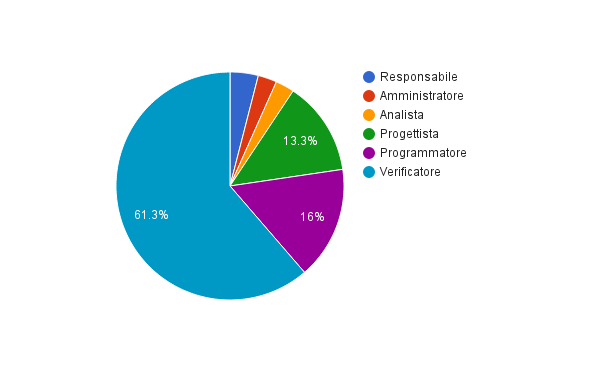
\includegraphics[width=0.9\textwidth]{../immagini/nuoviGrafici/oreFaseVerifica.png}
\caption{Ore per ruoli - Fase di \fVVt}
\end{figure}
\begin{figure}[h]
\centering
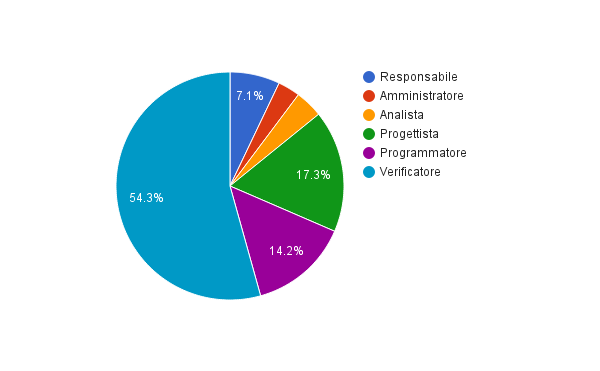
\includegraphics[width=0.9\textwidth]{../immagini/nuoviGrafici/costoFaseVerifica.png}
\caption{Costi per ruoli - Fase di \fVVt}
\end{figure}
\FloatBarrier
%----------------------------------------------------------------------------------------------
\subsection{Totali}
%----------------------------------------------------------------------------------------------
\subsubsection{Ore rendicontate}
\subsubsubsection{Suddivisione del lavoro}
Le ore totali rendicontate dedicate da ciascun componente all’intero \gloxy{progetto} saranno le seguenti:
%tabella suddivisione
\begin{table}[h]
\begin{center}
\begin{tabular}{|c|c|c|c|c|c|c|c|}
\hline Nome & Re & Am & An & Pt & Pr & Ve & Ore totali\\
\hline
\gma & - & 4 & 2 & 41 & 23 & 31 & 101 \\
\ao & - & - & 2 & 49 & 35 & 15 & 101 \\
\mb & 3 & - & 3 & 47 & 26 & 22 & 101 \\
\dm & 3 & - & - & 49 & 22 & 26 & 100 \\
\gmi & 6 & - & 3 & 34 & 3 & 54 & 100 \\
\sm & 3 & 4 & - & 51 & 10 & 33 & 101 \\
\fv & - & 2 & 5 & 34 & 9 & 51 & 101 \\
\hline Totale ruoli & 15 & 10 & 15 & 305 & 128 & 232 & 705 \\
\hline
\end{tabular}
\caption{Ore per ruolo - Totali rendicontate}
\end{center}
\end{table}
\FloatBarrier
I valori vengono riassunti nel seguente grafico:
\begin{figure}[htbp]
\centering
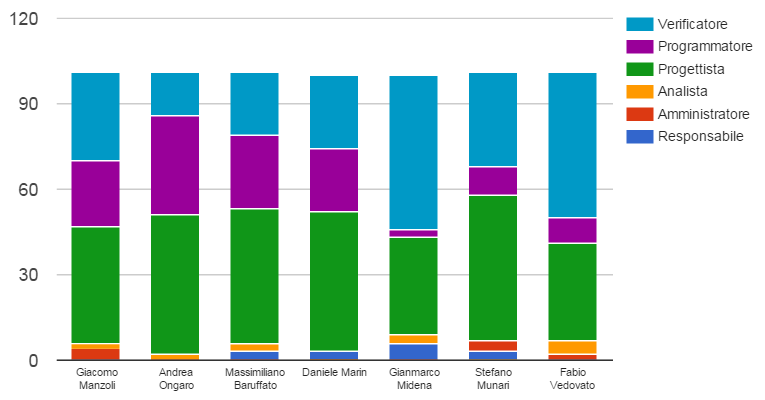
\includegraphics[width=1\textwidth]{../immagini/nuoviGrafici/componenti/oreCompTotaliRendicontate.png}
\caption{Ore per componente - Totali rendicontate}
\end{figure}
\FloatBarrier
\subsubsubsection{Prospetto economico}
La totalità delle ore rendicontate e il costo del \gloxy{progetto} a carico del \gloxy{Committente} sono riportati nella seguente tabella:
\begin{table}[h]
\begin{center}
\begin{tabular}{|m{3cm}|m{1.5cm}|m{1.5cm}|}
\hline Ruolo & Ore & Costo (\euro) \\
\hline
\rRPt & 15 & 450 \\
\rAPt & 10 & 200 \\
\rAt & 15 & 375 \\
\rPt & 305 & 6710 \\
\rpt & 128 & 1920 \\
\rVt & 232 & 3480 \\
\hline
Totale & 705 & 13135 \\
\hline
\end{tabular}
\caption{Prospetto economico - Totale, solo ore rendicontate}\label{tabellaTotale}
\end{center}
\end{table}
\FloatBarrier
I seguenti grafici illustrano rispettivamente come ciascun ruolo abbia influito sul totale delle ore e dei costi per l'intero \gloxy{progetto}.
%grafico a torta dei costi e delle ore
\begin{figure}[h]
\centering
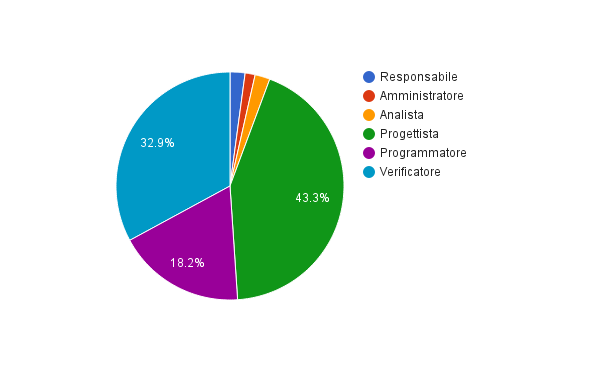
\includegraphics[width=0.9\textwidth]{../immagini/nuoviGrafici/oreTotaliSenzaAnalisi.png}
\caption{Ore per ruoli - Totali, rendicontati}
\end{figure}
\begin{figure}[h]
\centering
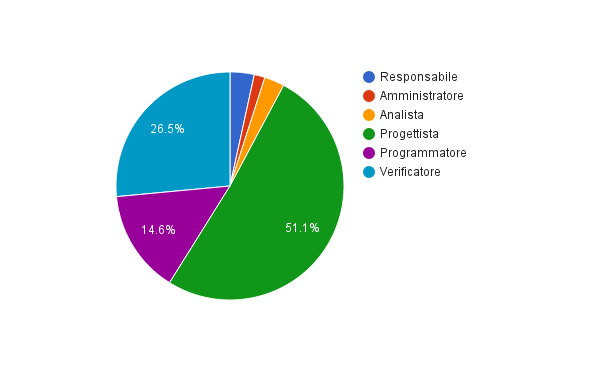
\includegraphics[width=0.9\textwidth]{../immagini/nuoviGrafici/costoTotaleSenzaAnalisi.png}
\caption{Costi per ruoli - Totali, rendicontati}
\end{figure}
\FloatBarrier
%----------------------------------------------------------------------------------------------
\subsubsection{Conclusioni}
Il costo totale per la realizzazione del \gloxy{progetto} è di \textbf{13135}\euro~ come riportato nella tabella \ref{tabellaTotale}.
